\documentclass[a4paper,twoside,11pt]{mwrep}
\usepackage[utf8]{inputenc}
\usepackage[T1]{fontenc}
\usepackage{polski}
\usepackage{graphicx}
\usepackage{xcolor}
\usepackage{hyperref}
\usepackage{amsmath}
\usepackage{amsthm}
\usepackage{amssymb}
\usepackage{bm}
\usepackage{enumitem}
\usepackage{mathrsfs}
\usepackage{tikz}
\usepackage{float}


\newcommand{\R}{{\mathbb R}}
\newcommand{\Z}{{\mathbb Z}}
\newcommand{\N}{{\mathbb N}}
\newcommand{\Q}{{\mathbb Q}}
\newcommand{\C}{{\mathbb C}}
\newcommand{\M}{{\textnormal{M}}}

\title{Dokumentacja aplikacji}
\author{Kamil Jarkowski, Damian Forma, Paweł Drzyzga}
\date{\today}

\begin{document}

\maketitle

\chapter{Wprowadzenie}

Aplikacja ta jest narzędziem służącym do:
\begin{itemize}
    \item Obliczania średnicy zbiorów,
    \item Obliczania odległości między zbiorami,
    \item (eksperymentalnie) Rysowania kul otwartych, domkniętych, jak i sfer w przestrzeni dwuwymiarowej.
\end{itemize}

Sama aplikacja została udostepniona przy pomocy oficjalnej strony streamowej pod linkiem \url{https://kursapp-pg9qzqkjjdkuyezpwiurdn.streamlit.app/}. Cały kod źródłowy aplikacji jest dostępny na platformie GitHub pod adresem \url{https://github.com/Qertal/KursStreamlit/tree/main/projekt_topo}.

\chapter{Pierwsze wejście na stronę aplikacji}

Możliwe, że pierwsze wejście na stronę aplikacji będzie trwało dłużej niż zwykle. Jest to spowodowane tym, że aplikacja jest uruchamiana na serwerze, a nie lokalnie. Dodatkowo, możliwe, że aplikacja będzie w stanie uśpienia \ref{rys:usp}. Wtedy wystarczy kliknąć przycisk z napisem \textit{Yes, get this app back up!}, a aplikacja zostanie uruchomiona ponownie.

%\includegraphics[]{Obraz1.png}

\begin{figure}[H] 
    \centering
    \includegraphics[width=0.8\textwidth]{figure/Obraz1.png}
    \caption{Uśpiona aplikacja}\label{rys:usp}
\end{figure}

\section{Strona główna aplikacji}

Na stronie głównej aplikacji \ref{rys:sg} znajdują się wypisani autorzy, a także po lewej stronie mały panel nawigacyjny, który pozwala na przejście do poszczególnych sekcji aplikacji, poprzez kliknięcie w odpowwiednią część. Warto zwrócić uwagę, że w każdej chwili można wrócić do strony głównej klikając przycisk \textit{Strona główna}. 

\begin{figure}[H] 
    \centering
    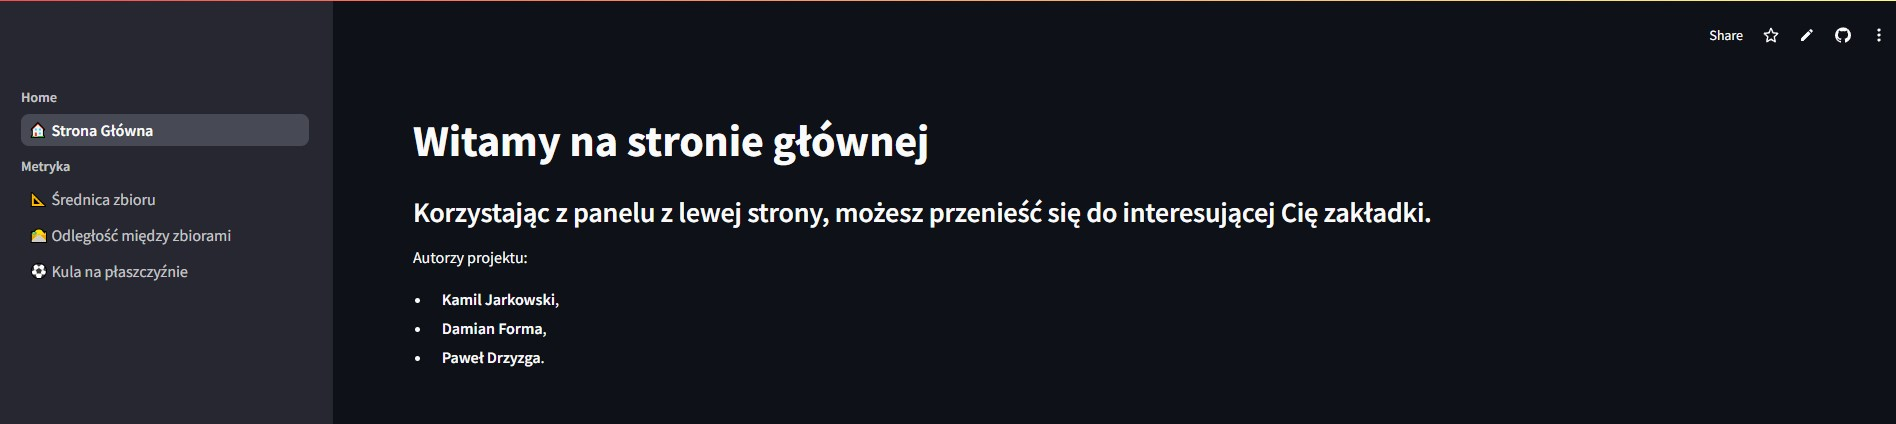
\includegraphics[width=0.8\textwidth]{figure/Screenshot_1.jpg}
    \caption{Strona główna}\label{rys:sg}
\end{figure}

Przejdźmy do pierwszej sekcji, a mianowicie do \textit{Średnica zbioru}.

\chapter{Średnica zbioru}

Klikając w przycisk \textit{Średnica zbioru} w polu nawigacji, przenosi nas na stronę \ref{rys:sz}, gdzie możemy skorzystać z kalkulatora średnicy zbioru. 

\begin{figure}[H] 
    \centering
    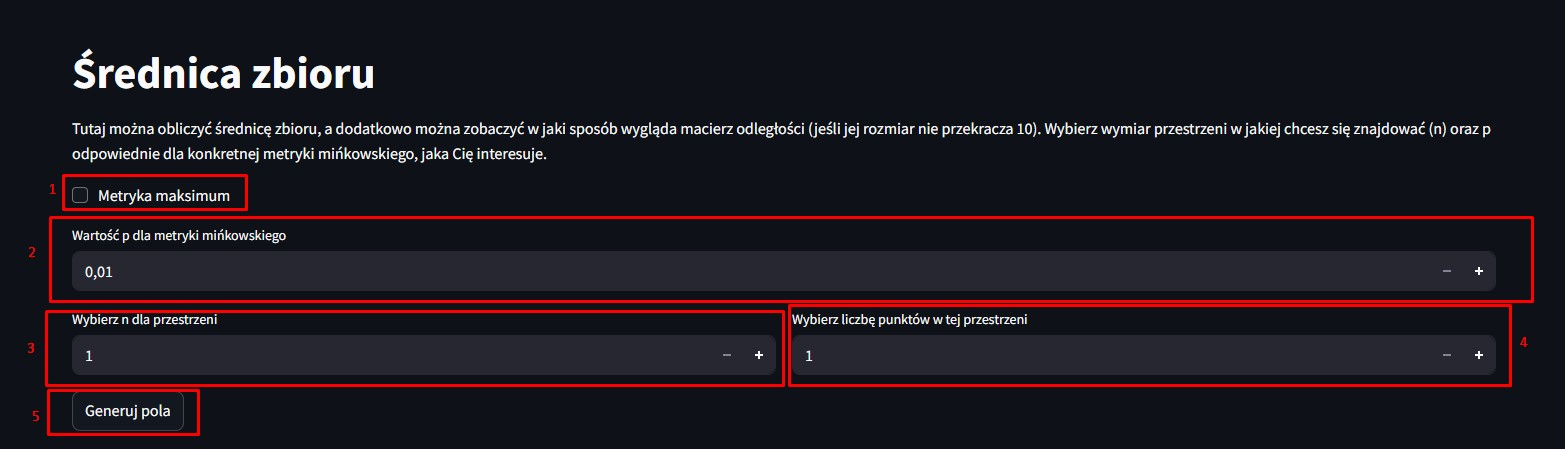
\includegraphics[width=0.8\textwidth]{figure/Screenshot_2.jpg}
    \caption{Strona główna}\label{rys:sz}
\end{figure}

Możemy zauważyć, różne sposoby interakcji ze stroną (numerki z listy poniżej są zgodne z numerkami na rysunku):
\begin{enumerate}
    \item W tym miejscu, możemy wybrać, czy metryka z której chcemy skorzystać, jest to metryka Czebyszewa, z racji na jej utrudnioną w sposobie zapisu symbolikę, została ona odizolowana od reszty, od klasycznego wyboru rodzaju metryki.
    \item Jeśli nie zdecydujemy się na wybór metryki Czebyszewa, możemy określić jakie użyjemy p ($p\in\R_+$) dla metryki Minkowskiego, czyli $d(x,y)=\left(\sum_{i=1}^n |x_i-y_i|^p\right)^{1/p}$. Możliwe jest wybranie wartości $p < 1$, co skutkuje użyciem wzoru $d(x,y)=\left(\sum_{i=1}^n |x_i-y_i|^p\right)$. W momencie gdy wybierzemy metrykę Czebyszewa, pole to automatycznie znika.
    \item W tym miejscu wybieramy wymiary przestrzeni, w której będziemy pracować. Czyli chodzi konkretnie o $n$ dla przestrzeni $\R^n$ ($n\in\N\backslash \{0\} $).
    \item Tutaj wybieramy ile punktów będzie w naszej przestrzeni. Wybierając $>10$ punktów, na sam koniec, nie zostanie wyświetlona macierz odległości, z racji na jej rozmiar. Warto mieć to na uwadzę.
    \item Na koniec mamy przycisk \textit{Generuj pola}, który generuje pola, które są potrzebne do wpisania punktów. Ciekawą opcją jaka została wprowadzona jest to, że pola zostają automatycznie uzupełnione losowymi liczbami całkowitymi z przedzlału $[-15,15]$, gdyby ktoś chciał szybko sprawdzić działanie aplikacji. Oczywiście możliwa jest edycja tych pól, w celu wpisania własnych punktów, gdzie współrzędne punktów muszą być liczbami całkowitymi.
\end{enumerate}

\end{document}
